\documentclass[main.tex]{subfiles}

\begin{document}

\section*{\Huge\textcolor{mantis}{Linear Regression}}
\addcontentsline{toc}{section}{Linear Regression}
\vspace{-0.3cm}
{\large\textit{Practical Guide: Methods, Formulas, and When to Use Them}}
\vspace{0.5cm}

\section{The Problem}

Given data $(x_i, y_i)$, we want to predict $y$ from $x$ using a linear relationship:
$$Y = a + bX + \varepsilon$$
where $\varepsilon$ is noise. The goal: find estimators $\hat{a}, \hat{b}$ that minimize prediction error.

\textbf{Univariate}: $x \in \R$ (one predictor). \textbf{Multivariate}: $x \in \R^d$ (multiple predictors).

\section{Ordinary Least Squares (OLS)}

\subsection{The Objective}

Minimize the sum of squared vertical distances (residuals):
$$\hat{\mathcal{R}}_n = \frac{1}{n} \sum_{i=1}^{n} (y_i - \hat{y}_i)^2$$

\textbf{Why squared loss?} The optimal predictor under squared loss is the conditional mean $\E[y|x]$ - exactly what we want to estimate.

\subsection{Univariate Formulas}

Setting derivatives to zero and solving:

$$\boxed{\hat{b} = \frac{\sum_{i=1}^{n} (x_i - \bar{x})(y_i - \bar{y})}{\sum_{i=1}^{n} (x_i - \bar{x})^2} = \frac{\widehat{\Cov}(X, Y)}{\widehat{\Var}(X)}}$$

$$\boxed{\hat{a} = \bar{y} - \hat{b}\bar{x}}$$

\textbf{Interpretation}: The slope is covariance over variance. The line passes through $(\bar{x}, \bar{y})$.

\subsection{Matrix Form (Multivariate)}

For $n$ observations and $d$ features, stack into:
$$\mathbf{y} = \mathbf{X}\boldsymbol{\theta} + \boldsymbol{\varepsilon}$$
where $\mathbf{X} \in \R^{n \times d}$ is the design matrix (include a column of 1s for intercept).

\textbf{The OLS solution}:
$$\boxed{\hat{\boldsymbol{\theta}} = (\mathbf{X}^\top\mathbf{X})^{-1}\mathbf{X}^\top\mathbf{y}}$$

\textbf{Requirement}: Need $\text{rank}(\mathbf{X}) = d$ (full column rank), which requires $n \geq d$.

\subsection{Geometric View}

$\hat{\mathbf{y}} = \mathbf{X}\hat{\boldsymbol{\theta}}$ is the orthogonal projection of $\mathbf{y}$ onto the column space of $\mathbf{X}$. The residuals $\mathbf{y} - \hat{\mathbf{y}}$ are perpendicular to all columns of $\mathbf{X}$.

\section{Key Properties of OLS}

\subsection{Residual Properties (Always Hold)}

From the optimization:
\begin{itemize}
    \item $\sum \varepsilon_i = 0$ - residuals have zero mean
    \item $\Cov(X, \varepsilon) = 0$ - residuals uncorrelated with predictors
\end{itemize}

\subsection{Classical Assumptions (For Inference)}

\begin{enumerate}
    \item \textbf{Linearity}: $\mathbf{y} = \mathbf{X}\boldsymbol{\theta} + \boldsymbol{\varepsilon}$
    \item \textbf{Exogeneity}: $\E[\boldsymbol{\varepsilon} | \mathbf{X}] = \mathbf{0}$
    \item \textbf{Spherical errors}: $\Var(\boldsymbol{\varepsilon}) = \sigma^2 \mathbf{I}_n$ (homoskedasticity, no autocorrelation)
    \item \textbf{Full rank}: $\text{rank}(\mathbf{X}) = d$
    \item \textbf{Normality} (for exact inference): $\boldsymbol{\varepsilon} \sim \mathcal{N}(\mathbf{0}, \sigma^2\mathbf{I})$
\end{enumerate}

\subsection{Under These Assumptions}

\begin{itemize}
    \item \textbf{Unbiased}: $\E[\hat{\boldsymbol{\theta}}] = \boldsymbol{\theta}$
    \item \textbf{Variance}: $\Var(\hat{\boldsymbol{\theta}}) = \sigma^2 (\mathbf{X}^\top\mathbf{X})^{-1}$
    \item \textbf{BLUE}: Best Linear Unbiased Estimator (Gauss-Markov theorem)
    \item \textbf{Distribution}: $\hat{\boldsymbol{\theta}} \sim \mathcal{N}(\boldsymbol{\theta}, \sigma^2(\mathbf{X}^\top\mathbf{X})^{-1})$
\end{itemize}

\subsection{Estimating $\sigma^2$}

$$\hat{\sigma}^2 = \frac{\text{RSS}}{n-d} = \frac{\sum(y_i - \hat{y}_i)^2}{n-d}$$

The denominator is $n-d$ (not $n$) to make this unbiased.

\section{Inference: Tests and Confidence Intervals}

\subsection{$t$-Test for Individual Coefficients}

Test $H_0: \theta_j = 0$:
$$t_j = \frac{\hat{\theta}_j}{\text{se}(\hat{\theta}_j)} \sim t_{n-d}$$
where $\text{se}(\hat{\theta}_j) = \hat{\sigma}\sqrt{[(\mathbf{X}^\top\mathbf{X})^{-1}]_{jj}}$.

\textbf{Confidence interval}: $\hat{\theta}_j \pm t_{n-d, \alpha/2} \cdot \text{se}(\hat{\theta}_j)$

\subsection{$F$-Test for Multiple Coefficients}

Test whether a group of coefficients are jointly zero:
$$F = \frac{(\text{RSS}_{\text{reduced}} - \text{RSS}_{\text{full}})/q}{\text{RSS}_{\text{full}}/(n-d)} \sim F_{q, n-d}$$
where $q$ = number of coefficients being tested.

\section{Bias-Variance Tradeoff}

\subsection{MSE Decomposition}

$$\text{MSE}(\hat{\theta}) = \text{Bias}(\hat{\theta})^2 + \text{Var}(\hat{\theta})$$

For prediction:
$$\E[(y_0 - \hat{y}_0)^2] = \underbrace{\sigma^2}_{\text{irreducible}} + \underbrace{\text{Bias}^2}_{\text{underfitting}} + \underbrace{\text{Variance}}_{\text{overfitting}}$$

\subsection{Practical Implications}

\begin{itemize}
    \item \textbf{High bias (underfitting)}: Model too simple, both train and test error high
    \item \textbf{High variance (overfitting)}: Model too complex, low train error but high test error
    \item \textbf{Solution}: Regularization trades bias for reduced variance
\end{itemize}

\begin{center}
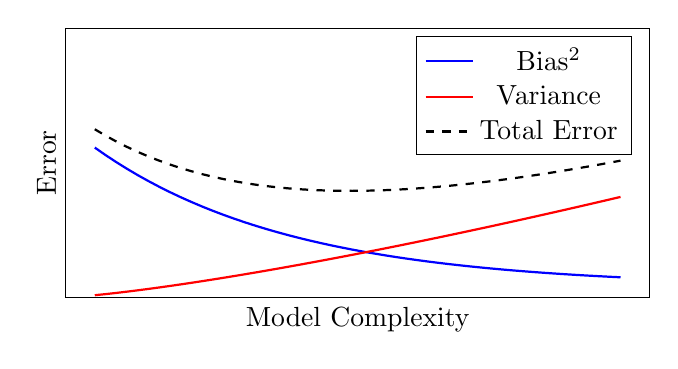
\begin{tikzpicture}
\begin{axis}[
    width=9cm, height=5cm,
    xlabel={Model Complexity}, ylabel={Error},
    xmin=0, xmax=10, ymin=0, ymax=5,
    xtick=\empty, ytick=\empty,
    legend pos=north east,
]
\addplot[domain=0.5:9.5, samples=50, color=blue, thick] {3*exp(-0.3*x) + 0.2};
\addplot[domain=0.5:9.5, samples=50, color=red, thick] {0.1*x^1.3};
\addplot[domain=0.5:9.5, samples=50, color=black, thick, dashed] {3*exp(-0.3*x) + 0.2 + 0.1*x^1.3 + 0.3};
\legend{Bias$^2$, Variance, Total Error}
\end{axis}
\end{tikzpicture}
\end{center}

\section{Regularization Methods}

\subsection{Ridge Regression ($L_2$)}

$$\hat{\boldsymbol{\theta}}_{\text{ridge}} = \arg\min \left\{ \|\mathbf{y} - \mathbf{X}\boldsymbol{\theta}\|_2^2 + \lambda\|\boldsymbol{\theta}\|_2^2 \right\}$$

\textbf{Solution}: $\hat{\boldsymbol{\theta}}_{\text{ridge}} = (\mathbf{X}^\top\mathbf{X} + \lambda\mathbf{I})^{-1}\mathbf{X}^\top\mathbf{y}$

\textbf{Properties}:
\begin{itemize}
    \item Biased but lower variance than OLS
    \item Shrinks coefficients toward zero (but never exactly zero)
    \item Always invertible (even when $d > n$)
    \item Larger $\lambda$ = more shrinkage
\end{itemize}

\textbf{When to use}: Multicollinearity, $d$ large relative to $n$, want stable predictions.

\subsection{Lasso ($L_1$)}

$$\hat{\boldsymbol{\theta}}_{\text{lasso}} = \arg\min \left\{ \frac{1}{2n}\|\mathbf{y} - \mathbf{X}\boldsymbol{\theta}\|_2^2 + \lambda\|\boldsymbol{\theta}\|_1 \right\}$$

\textbf{Properties}:
\begin{itemize}
    \item No closed-form solution (use coordinate descent)
    \item \textbf{Produces sparse solutions}: some $\hat{\theta}_j = 0$ exactly
    \item Performs automatic variable selection
\end{itemize}

\textbf{When to use}: Feature selection, believe only a few features matter.

\subsection{Elastic Net}

$$\hat{\boldsymbol{\theta}}_{\text{EN}} = \arg\min \left\{ \|\mathbf{y} - \mathbf{X}\boldsymbol{\theta}\|_2^2 + \lambda_1\|\boldsymbol{\theta}\|_1 + \lambda_2\|\boldsymbol{\theta}\|_2^2 \right\}$$

\textbf{When to use}: Want sparsity (Lasso) but have correlated features (Ridge helps select groups together).

\subsection{Choosing $\lambda$}

Use \textbf{cross-validation}: select $\lambda$ minimizing CV error.

\section{Model Evaluation}

\subsection{$R^2$ (Coefficient of Determination)}

$$R^2 = 1 - \frac{\text{RSS}}{\text{TSS}} = 1 - \frac{\sum(y_i - \hat{y}_i)^2}{\sum(y_i - \bar{y})^2}$$

\begin{itemize}
    \item $R^2 = 1$: perfect fit
    \item $R^2 = 0$: no better than predicting $\bar{y}$
    \item \textbf{Problem}: Always increases with more features (even noise)
\end{itemize}

\subsection{Adjusted $R^2$}

$$\bar{R}^2 = 1 - \frac{n-1}{n-d}(1 - R^2)$$

Penalizes for number of parameters. Can decrease when adding useless features.

\subsection{Information Criteria}

\textbf{AIC}: $-2\log L + 2d$ \quad (efficient, minimizes prediction error)

\textbf{BIC}: $-2\log L + d\log n$ \quad (consistent, finds true model, penalizes more)

Lower is better. For linear regression: $\text{AIC} \approx n\log(\text{RSS}/n) + 2d$.

\subsection{Cross-Validation}

\begin{enumerate}
    \item Split data into $k$ folds
    \item For each fold: train on rest, test on fold
    \item Average the $k$ test errors
\end{enumerate}

Typical: $k = 5$ or $k = 10$. Gold standard for model selection.

\section{Common Problems and Solutions}

\subsection{Multicollinearity}

\textbf{Symptom}: Predictors highly correlated $\Rightarrow$ $\mathbf{X}^\top\mathbf{X}$ nearly singular.

\textbf{Detection}: Variance Inflation Factor: $\text{VIF}_j = 1/(1 - R_j^2)$. VIF $> 10$ is problematic.

\textbf{Solutions}:
\begin{itemize}
    \item Ridge regression (stabilizes)
    \item Remove redundant features
    \item Principal Component Regression (PCR)
\end{itemize}

\subsection{Heteroskedasticity}

\textbf{Symptom}: $\Var(\varepsilon_i)$ varies across observations.

\textbf{Detection}: Breusch-Pagan test (regress $\hat{\varepsilon}_i^2$ on $\mathbf{x}_i$).

\textbf{Solutions}:
\begin{itemize}
    \item Robust standard errors (sandwich estimator)
    \item Weighted Least Squares / GLS
\end{itemize}

\subsection{$d > n$ (More Features than Observations)}

OLS doesn't work ($\mathbf{X}^\top\mathbf{X}$ not invertible).

\textbf{Solutions}: Ridge, Lasso, Elastic Net, PCR.

\section{Advanced Methods}

\subsection{Principal Component Regression (PCR)}

\begin{enumerate}
    \item Run PCA on $\mathbf{X}$, keep top $k$ components
    \item Regress $\mathbf{y}$ on the $k$ principal components
\end{enumerate}

\textbf{When to use}: High-dimensional, want to reduce dimension without explicit sparsity.

\subsection{Kernel Ridge Regression}

Replace inner products with kernel function $k(\mathbf{x}, \mathbf{x}')$:

$$\hat{y}(\mathbf{x}) = \mathbf{k}(\mathbf{x})^\top(\mathbf{K} + \lambda\mathbf{I})^{-1}\mathbf{y}$$

Common kernels:
\begin{itemize}
    \item Linear: $k(\mathbf{x}, \mathbf{x}') = \mathbf{x}^\top\mathbf{x}'$
    \item RBF: $k(\mathbf{x}, \mathbf{x}') = \exp(-\|\mathbf{x} - \mathbf{x}'\|^2/2\sigma^2)$
\end{itemize}

\textbf{When to use}: Nonlinear relationships, moderate $n$ (scales $O(n^3)$).

\subsection{Quantile Regression}

Estimates conditional quantiles instead of mean. Uses check loss:
$$\rho_\tau(u) = u(\tau - \mathbf{1}_{u < 0})$$

\textbf{When to use}: Interested in median or other quantiles, robust to outliers.

\section{Method Selection Guide}

\begin{center}
\small
\begin{tabular}{lll}
\hline
\textbf{Situation} & \textbf{Method} & \textbf{Reason} \\
\hline
$n \gg d$, no issues & OLS & Simple, unbiased, BLUE \\
Multicollinearity & Ridge & Stabilizes coefficients \\
Want feature selection & Lasso & Produces exact zeros \\
Correlated features + sparsity & Elastic Net & Best of both \\
$d > n$ & Ridge/Lasso/EN & OLS undefined \\
Nonlinear patterns & Kernel methods & Implicit feature expansion \\
Outliers in $y$ & Quantile regression & Robust to outliers \\
Heteroskedasticity & Robust SE or GLS & Correct inference \\
\hline
\end{tabular}
\end{center}

\section{Quick Reference: Key Formulas}

\begin{align*}
\text{OLS (univariate):} \quad & \hat{b} = \frac{\widehat{\Cov}(X,Y)}{\widehat{\Var}(X)}, \quad \hat{a} = \bar{y} - \hat{b}\bar{x} \\[6pt]
\text{OLS (matrix):} \quad & \hat{\boldsymbol{\theta}} = (\mathbf{X}^\top\mathbf{X})^{-1}\mathbf{X}^\top\mathbf{y} \\[6pt]
\text{Ridge:} \quad & \hat{\boldsymbol{\theta}} = (\mathbf{X}^\top\mathbf{X} + \lambda\mathbf{I})^{-1}\mathbf{X}^\top\mathbf{y} \\[6pt]
\text{Variance:} \quad & \Var(\hat{\boldsymbol{\theta}}) = \sigma^2(\mathbf{X}^\top\mathbf{X})^{-1} \\[6pt]
\text{MSE:} \quad & \text{Bias}^2 + \text{Variance} \\[6pt]
R^2: \quad & 1 - \text{RSS}/\text{TSS} \\[6pt]
\text{Adjusted } R^2: \quad & 1 - \frac{n-1}{n-d}(1-R^2)
\end{align*}

\end{document}

